\documentclass[serif,mathserif]{beamer}
\usepackage{amsmath, amsfonts, epsfig, xspace}
\usepackage{algorithm,algorithmic}
\usepackage{pstricks,pst-node}
\usepackage{multimedia}
\usepackage[normal,tight,center]{subfigure}
\setlength{\subfigcapskip}{-.5em}
\usepackage{beamerthemesplit}
\usetheme{lankton-keynote}

\usepackage{mdframed}

\hypersetup{colorlinks}

\def\gw#1{gravitational wave#1 (GW#1)\gdef\gw{GW}}
\def\ns#1{neutron star#1 (NS#1)\gdef\ns{NS}}

%\titlegraphic{
\includegraphics[width=0.5\textwidth]{figures/cra.png}}

\begin{document}
\setbeamertemplate{caption}{\raggedright\insertcaption\par}

\title[BNS Bursts]{Searching For Gravitational Wave Bursts From
Binary Neutron Star Coalescence}
\author{James A. Clark}
\institute{Georgia Institute of Technology}
\date{} 

%\maketitle

\begin{frame}[plain]
\titlepage
\end{frame}

\begin{frame}
    \frametitle{This Talk}
    \tableofcontents
\end{frame} 

\section{GW Bursts From BNS Mergers}

\begin{frame}
    \frametitle{Burst Signals: Short}
\end{frame}

\begin{frame}
    \frametitle{Burst Signals: Short}
    \begin{figure}
        \centering
        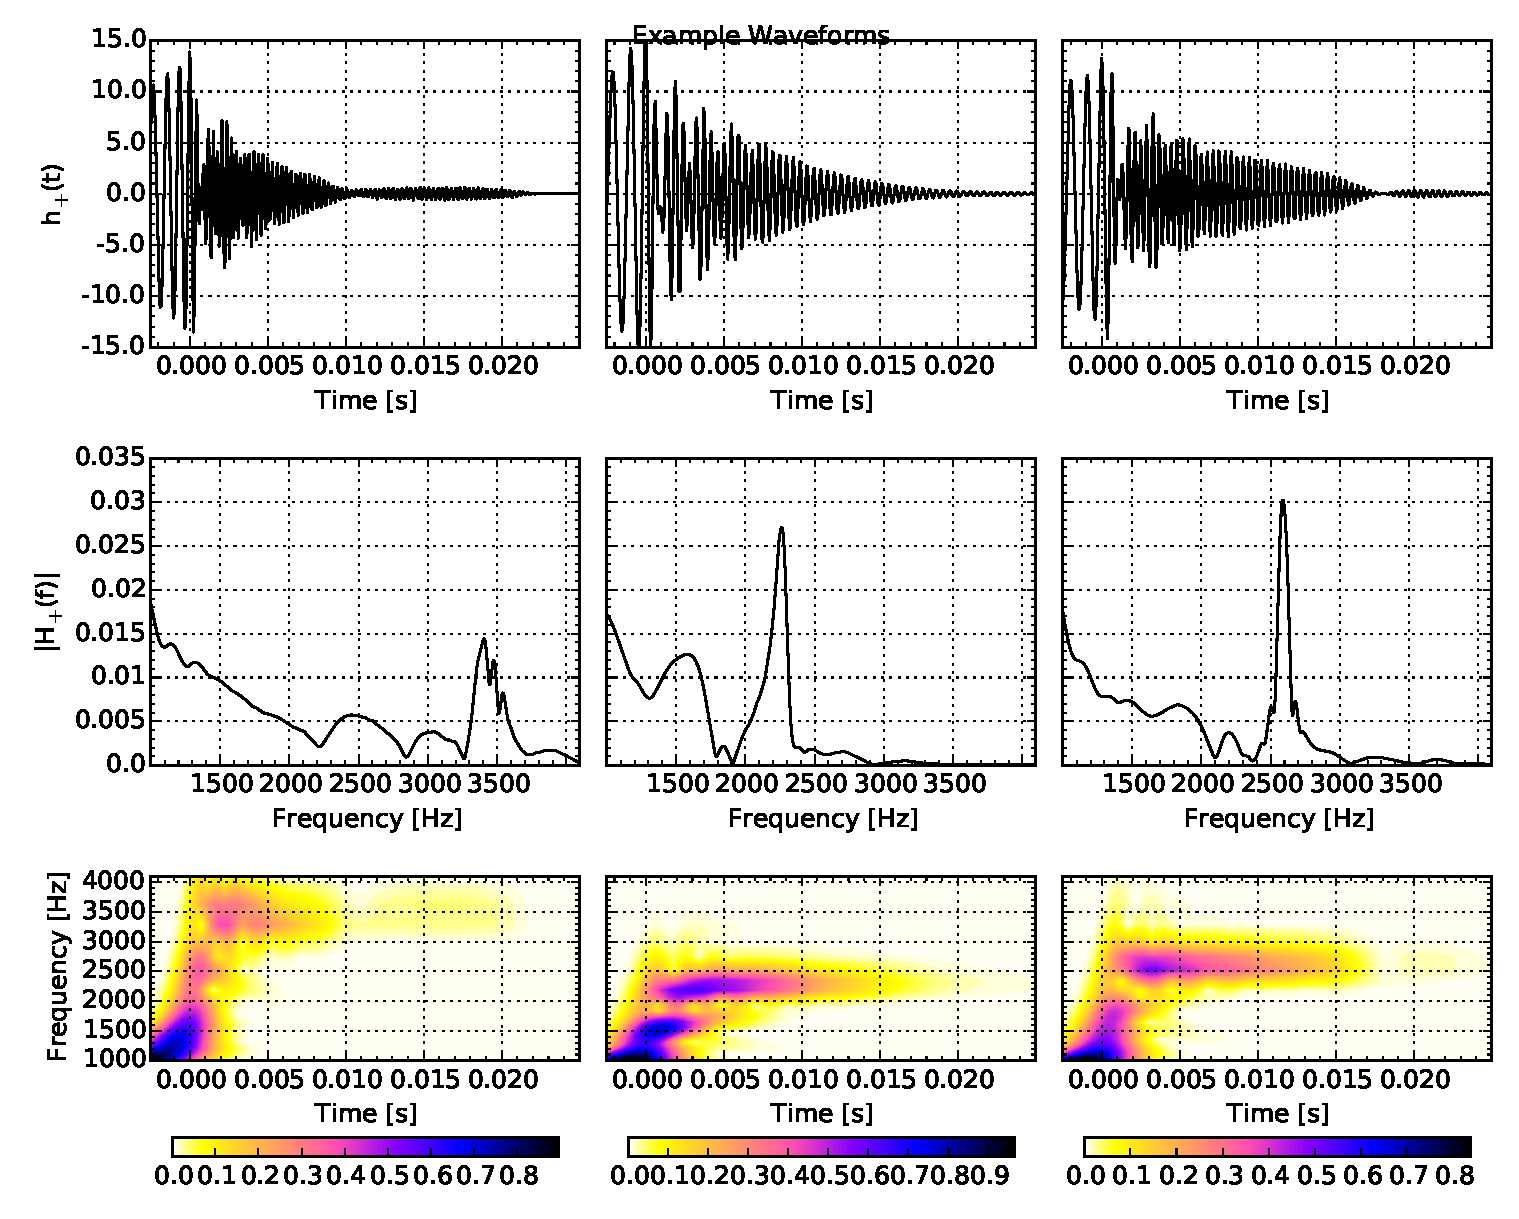
\includegraphics[width=0.9\columnwidth]{figures/example_waves.pdf}
    \end{figure}
\end{frame}

\begin{frame}
    \frametitle{Burst Signals: Long}
\end{frame}

\section{GW Burst Data Analysis}

\begin{frame}
    \frametitle{Basic Idea}
\end{frame}


\begin{frame}
    \frametitle{Detectability \& Frequency Recovery}

    \begin{columns}[]

        \column{0.6\textwidth}

        \begin{center}
            \vspace{-0.5cm}
            \begin{figure}
                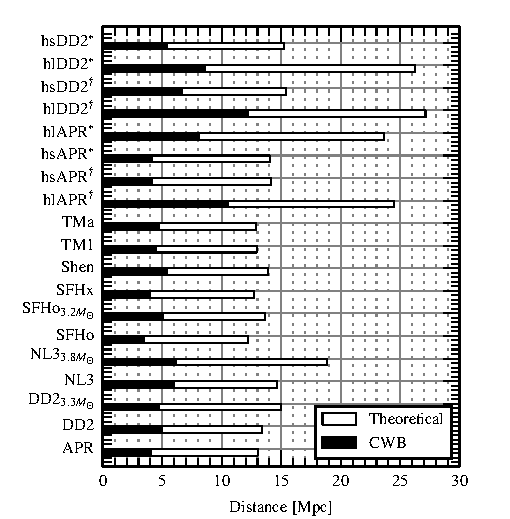
\includegraphics[width=\columnwidth]{figures/distances.pdf}
            \end{figure}
        \end{center}

        \column{0.6\textwidth}

        \begin{center}
            \vspace{-0.5cm}
            \begin{figure}
                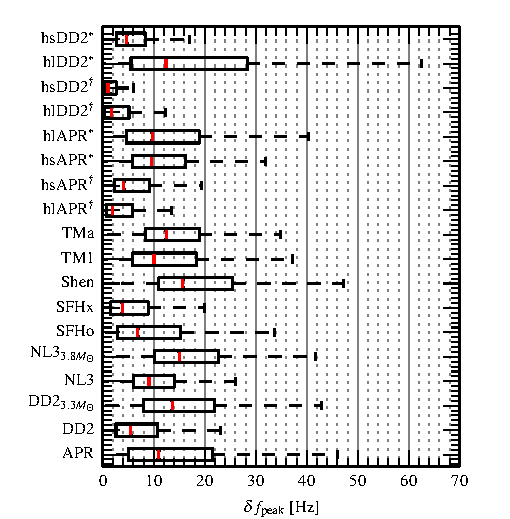
\includegraphics[width=\columnwidth]{figures/deltaFpeak.pdf}
            \end{figure}
        \end{center}

    \end{columns}

\end{frame}

\section{GW Burst Data Analysis: Future Prospects \& Development}

\begin{frame}
    \frametitle{Enhancements \& Bayesian Methods}
\end{frame}


\begin{frame}
    \frametitle{Propose: Principal Component Analysis Of Short Bursts}

    \begin{figure}
        \centering
        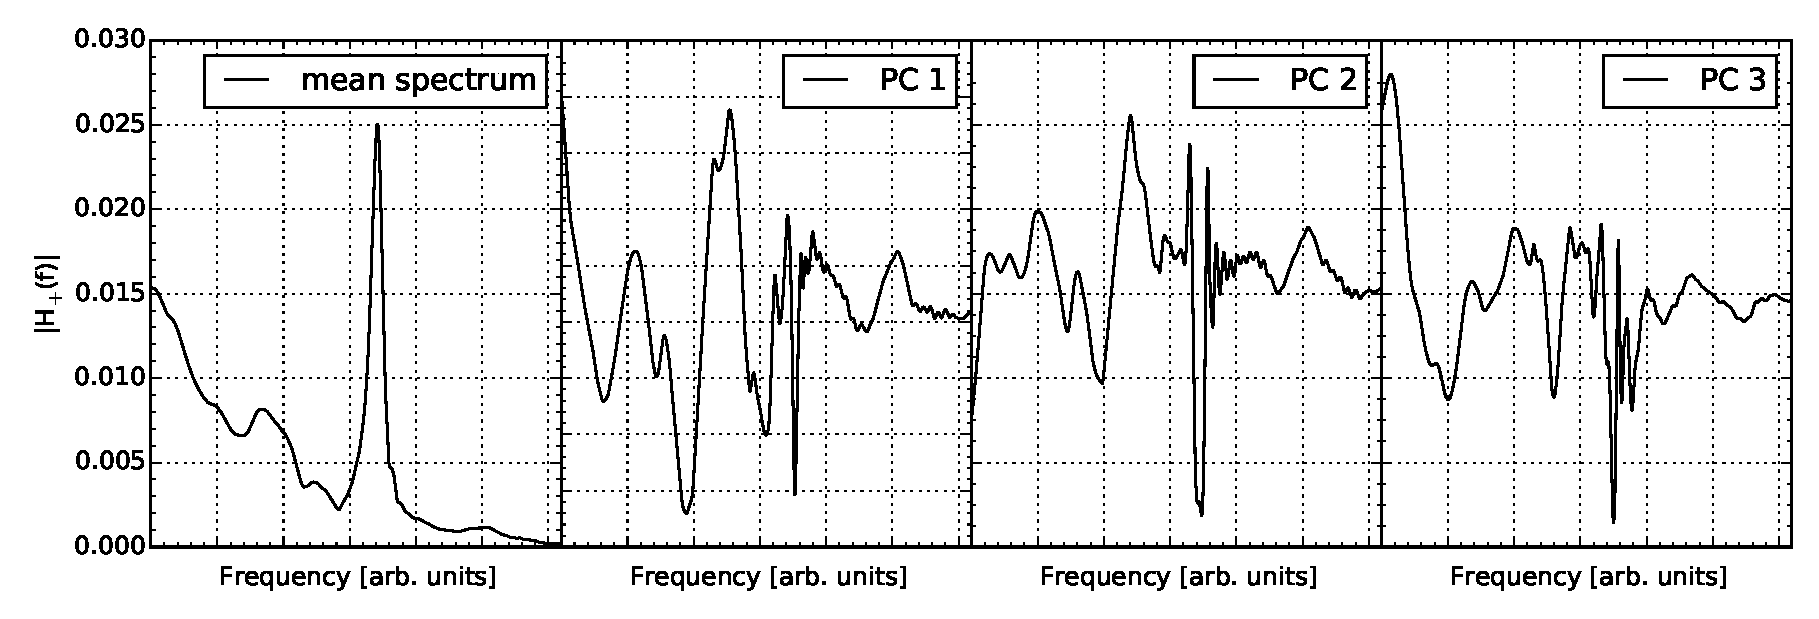
\includegraphics[width=\columnwidth]{figures/magnitude_pcs.pdf}
    \end{figure}

\end{frame}

\begin{frame}
    \frametitle{Prospects for PCA Of Short Bursts}

    \begin{columns}[]

        \column{0.5\textwidth}

        \begin{center}
            \vspace{-0.5cm}
            \begin{figure}
                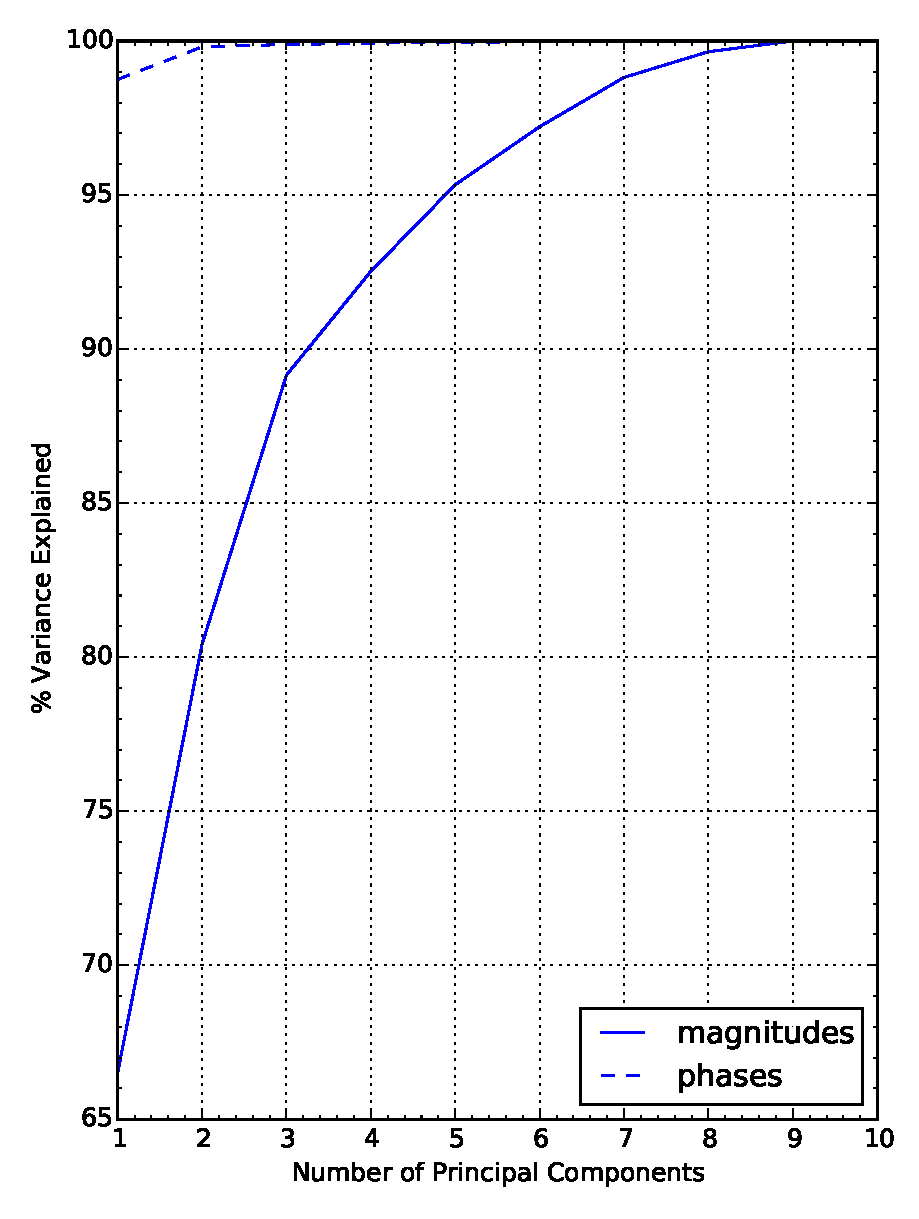
\includegraphics[width=\columnwidth]{figures/explained_variance.pdf}
            \end{figure}
        \end{center}

        \column{0.5\textwidth}

        \begin{center}
            \vspace{-0.5cm}
            \begin{figure}
                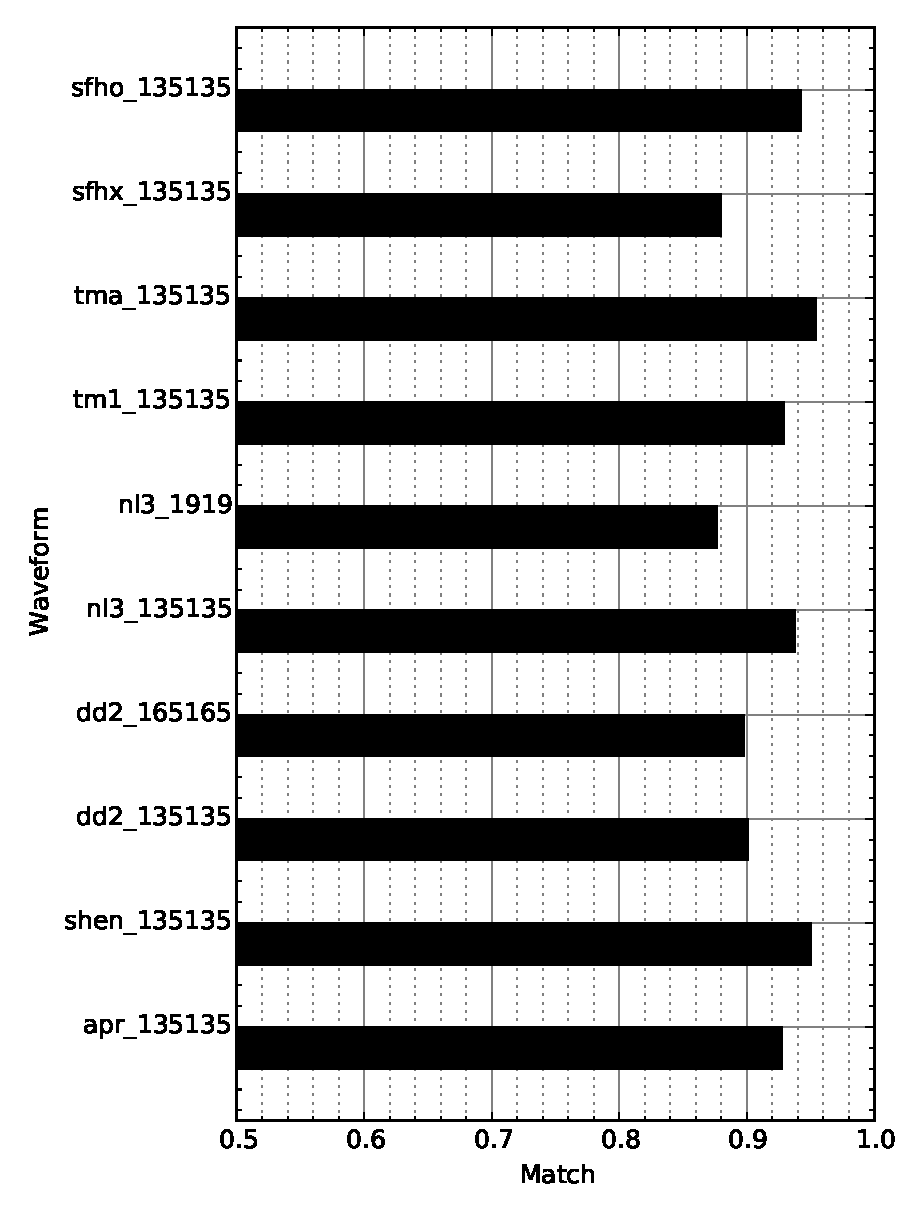
\includegraphics[width=\columnwidth]{figures/match_bars_exctestwav.pdf}
            \end{figure}
        \end{center}


    \end{columns}

\end{frame}

\begin{frame}
    \frametitle{Next Steps With PCA}
\end{frame}

\begin{frame}
    \frametitle{Searching For Long Bursts}
\end{frame}

\section{Summary \& Outlook}
\begin{frame}
    \frametitle{Summary}
\end{frame}

\appendix
\section{GW Burst Data Analysis: Future Prospects \& Development}

\begin{frame}
    \frametitle{Principal Component Analysis Of Short Bursts}



        \begin{center}
            \vspace{-0.5cm}
            \begin{figure}
                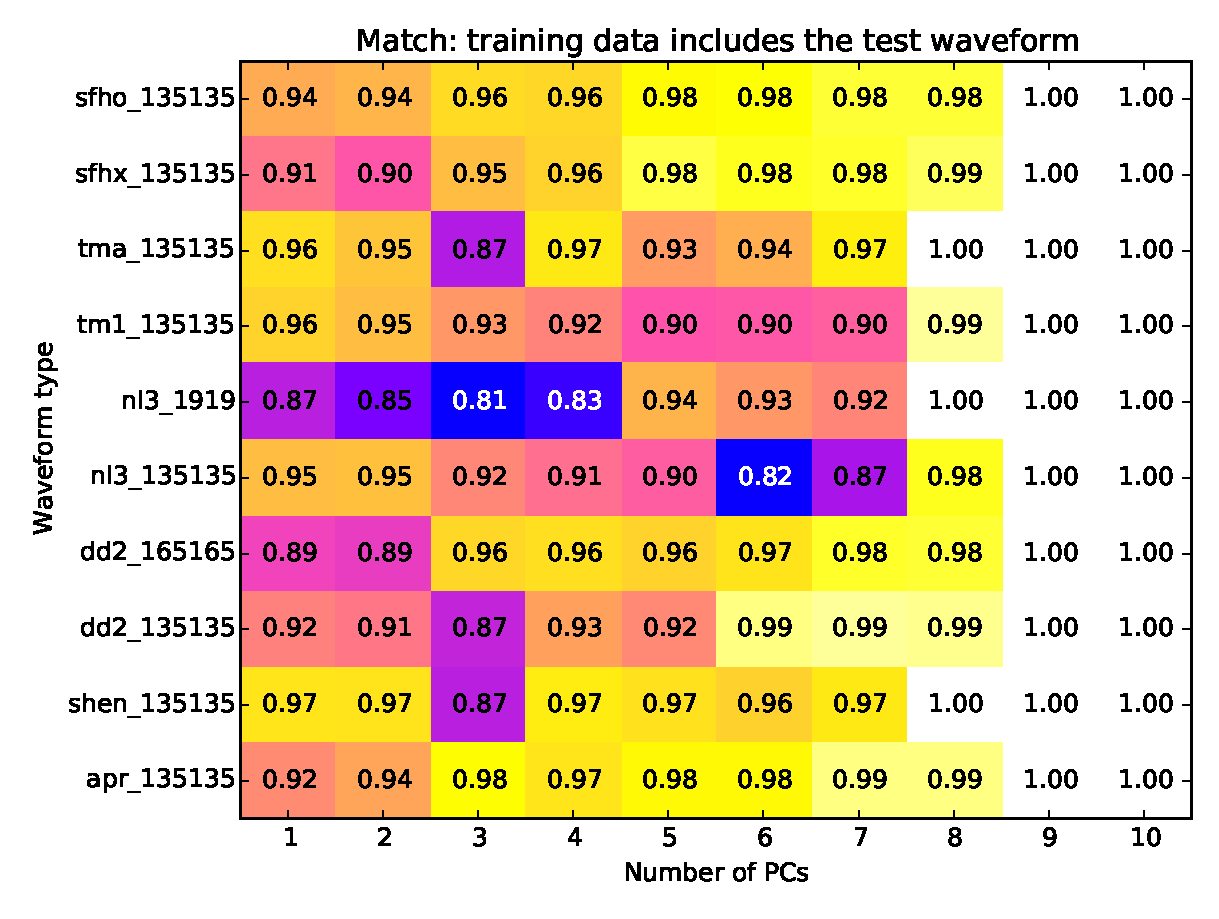
\includegraphics[width=\columnwidth]{figures/match_grid_inctestwav.pdf}
            \end{figure}
        \end{center}

\end{frame}

\begin{frame}
    \frametitle{Principal Component Analysis Of Short Bursts}

        \begin{center}
            \vspace{-0.5cm}
            \begin{figure}
                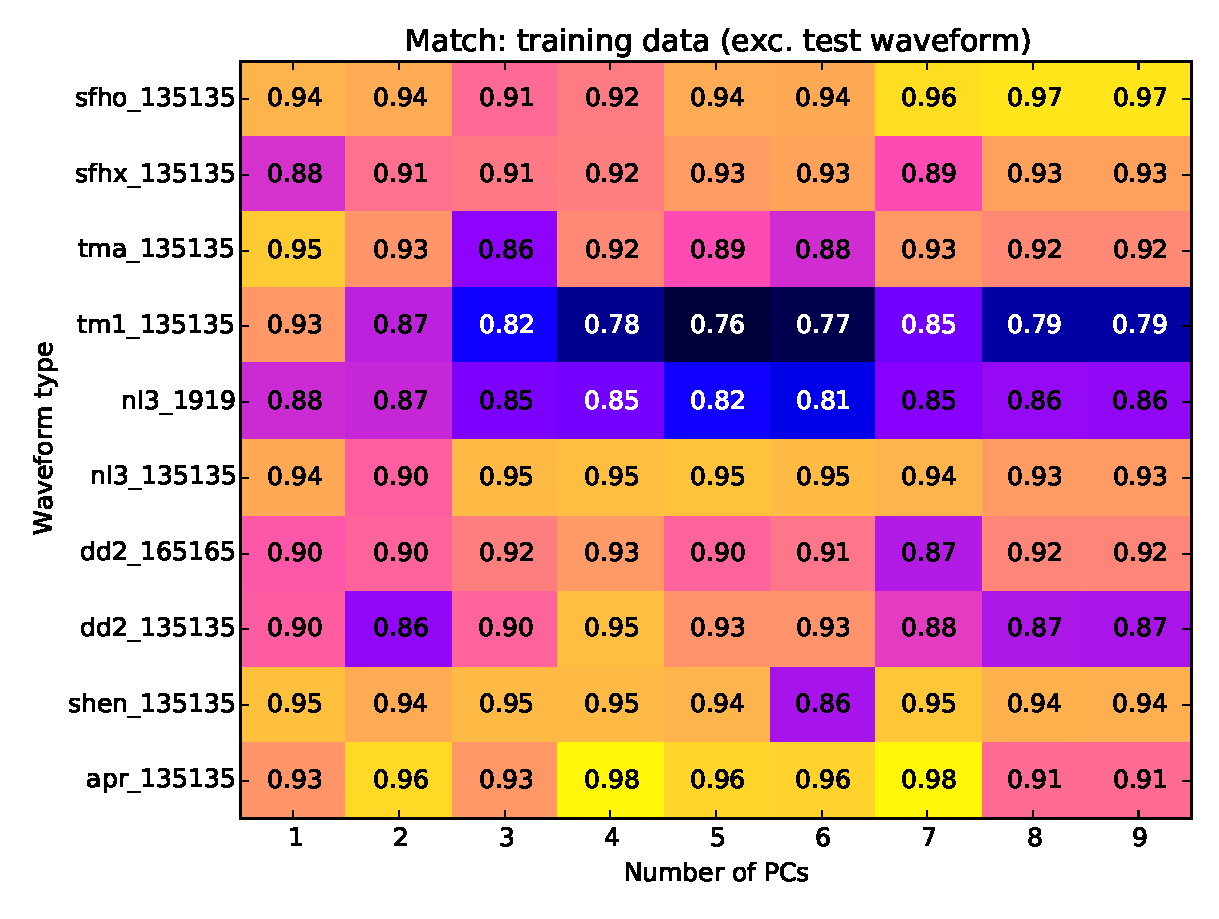
\includegraphics[width=\columnwidth]{figures/match_grid_exctestwav.pdf}
            \end{figure}
        \end{center}


\end{frame}

\end{document}

